\RequirePackage{fix-cm}
\documentclass[oneside, a4paper]{book}
\usepackage[a4paper,width=150mm,top=25mm,bottom=25mm,bindingoffset=6mm]{geometry}

% Required for inserting images
\usepackage{eso-pic,graphicx}
% misc
\usepackage{caption}
\DeclareCaptionType{equ}[][]
%\captionsetup[equ]{labelformat=empty}
\usepackage{subcaption}
\usepackage{multicol}
\usepackage{float}
\usepackage{adjustbox} % oversized table

% appendix
\usepackage[toc]{appendix}

% Default font to sans serif
\renewcommand{\familydefault}{\sfdefault}
\RequirePackage[T1]{fontenc} 
\RequirePackage[tt=false, type1=true]{libertine} 
\RequirePackage[varqu]{zi4} 
% \RequirePackage[libertine]{newtxmath}

% chapters and headers
\usepackage[Conny]{fncychap}

\usepackage{fancyhdr}
\pagestyle{fancy}
\renewcommand{\headrulewidth}{0.1pt}
\renewcommand{\chaptermark}[1]{\markboth{\MakeUppercase{\textsf{{#1}}}}{}}
\renewcommand{\sectionmark}[1]{\markright{\MakeUppercase{\textsf{\thesection\ #1}}}{} }

% section styling
\usepackage{titlesec}

% algorithms
\usepackage{algorithm}
\usepackage{algpseudocode}

% theorems and definitions
\usepackage{amsthm}
\newtheorem{definition}{Definition}

% better tables
\usepackage{tabu}

% FAT FONTS
\usepackage{bm} % bold fonts in math mode
\newcommand\fat[1]{{\boldmath{\textbf{#1}}}}
\newcommand\emphasis[1]{{\scshape\bfseries#1}}

% mathematical fonts and graphics
\usepackage{mathtools}
\usepackage{xfrac} % sfrac for diagonal slashes in fractions
\usepackage{amsfonts} % math fonts
\usepackage{amssymb} % more math symbols (supsetneq etc.)
\usepackage{dbnsymb}
\usepackage{dsfont} % math fonts
\usepackage{bbm} % mathbb fonts
\usepackage{mathrsfs} % fancy swirly font
\usepackage{gensymb} % degree sign

% draw graphs
\usepackage[inline]{asymptote}
\usepackage{qtree}
\usepackage{tikz}
\usetikzlibrary{calc}

% nicer fractions
\usepackage{xfrac}
% cancel terms
\usepackage{cancel}

% units
\usepackage{siunitx}

% plots
\usepackage{pgfplots}
\usepackage{pgfplotstable}
\usepgfplotslibrary{external}
\usepgfplotslibrary{patchplots}
\usepgfplotslibrary{groupplots}
\pgfplotsset{compat=1.18} 
\tikzexternalize[prefix=tikz,optimize=false]

% define the Spectral_r color scheme
\usepackage[table, dvipsnames]{xcolor}
\definecolor{Spectral0}{RGB}{158, 1, 66}
\definecolor{Spectral1}{RGB}{213, 62, 79}
\definecolor{Spectral2}{RGB}{244, 109, 67}
\definecolor{Spectral3}{RGB}{253, 174, 97}
\definecolor{Spectral4}{RGB}{254,224,139}
\definecolor{Spectral5}{RGB}{255,255,191}
\definecolor{Spectral6}{RGB}{230,245,152}
\definecolor{Spectral7}{RGB}{171,221,164}
\definecolor{Spectral8}{RGB}{102,204,204}
\definecolor{Spectral9}{RGB}{50,136,189}
\definecolor{Spectral10}{RGB}{94,79,162}
\pgfplotsset{
  colormap={Spectral_r}{
    rgb255(0cm)=(94,79,162)         % 0.0
    rgb255(1cm)=(50,136,189)        % 0.1
    rgb255(2cm)=(102,204,204)       % 0.2
    rgb255(3cm)=(171,221,164)       % 0.3
    rgb255(4cm)=(230,245,152)       % 0.4
    rgb255(5cm)=(255,255,191)       % 0.5
    rgb255(6cm)=(254,224,139)       % 0.6
    rgb255(7cm)=(253,174,97)        % 0.7
    rgb255(8cm)=(244,109,67)        % 0.8
    rgb255(9cm)=(213,62,79)         % 0.9
    rgb255(10cm)=(158,1,66)         % 1.0
    }
}


% get width of given text
\usepackage{calc}

% define a horizontal spacer
\newcommand\horizontalspacer[0]{\vspace{5pt}\noindent\textcolor{lightgray}{\rule{\textwidth}{1mm}}
\vspace{5pt}}

% clickable links
\usepackage{hyperref}
\hypersetup{
    colorlinks,
    citecolor=black,
    filecolor=black,
    linkcolor=black,
    urlcolor=black
}
\renewcommand{\itemautorefname}{Item}
% fancy boxes
\usepackage{fancybox}
\newcommand{\equationnamed}[2]{%
  \setlength{\fboxsep}{2pt} % padding inside box
  \setlength{\fboxrule}{0.01pt}
  \begin{center}
    \begin{minipage}{\textwidth}
      \begin{center}\textsc{#1}\end{center}
      #2
    \end{minipage}
  \end{center}
}
\newcommand{\equationnamedbox}[2]{%
  \setlength{\fboxsep}{5pt} % padding inside box
  \setlength{\fboxrule}{0.01pt}
  \begin{center}
    \fbox{
      \begin{minipage}{0.4\textwidth}
        \begin{center}\emphasis{#1}\end{center}
        #2
      \end{minipage}
    }
  \end{center}
}

% labels to enum items
\usepackage{enumitem}

\usepackage{array}

% make empty lines skip
% \usepackage{parskip}

% include pdfs 
\usepackage{pdfpages}

% code
\usepackage{minted}
\usepackage{listings}

% ~~~~~~~~~ TYPESETTING AND OTHER MACROS ~~~~~~~~~~~~~~~~~~~~~

\newenvironment{absolutelynopagebreak}
  {\par\nobreak\vfil\penalty0\vfilneg
   \vtop\bgroup}
  {\par\xdef\tpd{\the\prevdepth}\egroup
   \prevdepth=\tpd}

% ~~~~~~~~~ AFANCY CHAPTER HEADINGS ~~~~~~~~~~~~~~~~~~~~~~~~~~~
\makeatletter
\def\thickhrulefill{\leavevmode \leaders \hrule height 1ex \hfill \kern \z@}
\def\@makechapterhead#1{%
  %\vspace*{50\p@}%
  \vspace*{10\p@}%
  {\parindent \z@ \centering \reset@font
        \thickhrulefill\quad
        \scshape \@chapapp{} \thechapter
        \quad \thickhrulefill
        \par\nobreak
        \vspace*{10\p@}%
        \interlinepenalty\@M
        \hrule
        \vspace*{10\p@}%
        \Huge {\textbf{#1}} \par\nobreak
        \par
        \vspace*{10\p@}%
        \hrule
    \vskip 40\p@
    % \vskip 100\p@
  }}
\def\@makeschapterhead#1{%
  %\vspace*{50\p@}%
  \vspace*{10\p@}%
  {\parindent \z@ \centering \reset@font
        \thickhrulefill
        \par\nobreak
        \vspace*{10\p@}%
        \interlinepenalty\@M
        \hrule
        \vspace*{10\p@}%
        \Huge \bfseries #1\par\nobreak
        \par
        \vspace*{10\p@}%
        \hrule
    \vskip 40\p@
    % \vskip 100\p@
  }}

  \newcommand*{\@rowstyle}{}
  \newcommand*{\rowstyle}[1]{% sets the style of the next row
    \gdef\@rowstyle{#1}%
    \@rowstyle\ignorespaces%
  }
  \newcolumntype{=}{% resets the row style
    >{\gdef\@rowstyle{}}%
  }
  \newcolumntype{+}{% adds the current row style to the next column
    >{\@rowstyle}%
  }
  
\usepackage[pdftex,outline]{contour}

% ~~~~~~~~~ MATH MACROS ~~~~~~~~~~~~~~~~~~~~~~~~~~~~~~~~~~~~~~

% abs value macro
% \DeclarePairedDelimiter\abs{\lvert}{\rvert}
\newcommand\abs[1]{\left|#1\right|}
\newcommand\abss[1]{\left|\left|#1\right|\right|}
\newcommand\norm[1]{\left\lVert#1\right\rVert}
\newcommand\angled[1]{\left\langle#1\right\rangle}
\newcommand\round[1]{\left\lfloor#1\right\rceil}

\newcommand\dist[1]{\left|\left|#1\right|\right|}
\newcommand\arr[1]{\left\langle#1\right\rangle}
\newcommand\pdpi[0]{\frac{\partial}{\partial p_i}}

% define the laplace operator 
\newcommand*\Laplace{\mathop{}\!\mathbin\nabla^2}
\newcommand\vek[1]{\vec{\bm{#1}}}
\newcommand\nvek[1]{\hat{\vec{\bm{#1}}}}
\newcommand\mat[1]{{\mathds{#1}}}
\newcommand\br[1]{\left(#1\right)}

\DeclareMathOperator{\sgn}{sgn}
\DeclareMathOperator{\erf}{erf}

\DeclareMathOperator*{\argmax}{\arg\!\max}
\DeclareMathOperator*{\argmin}{\arg\!\min}

\newcommand\divergence{{\nabla\cdot}}


\author{Julian Karrer}
\title{Exercise 4: Constrained Optimization}

\begin{document}
\chapter{Hanging chain, the last episode: the Interior Point Method}
\equationnamedbox{Generic Inequality-Constrained QP}{
    \begin{align}
    \min_{x\in\mathds{R}^n} \quad & \frac{1}{2} x^T Q x + c^T x \\
    \text{s.t.}\quad & \forall j\in\mathds{N}_1^m \quad a_j^T x+b_j\geq 0
    \end{align}
}

\section{Type of Problem}
The problem is convex quadratic program with affine inequality constraints.

\section{Convexity of Barrier function}
The feasible set remains unchanged in this formulation, so convexity of the problem depends on the convexity of the objective: 
\begin{equation}
  f^{[k]}(x) =  f(x) - \tau^{[k]} \sum_{j=1}^m \log\br{a_j^T x + b_j}
\end{equation}

Assuming $f(x)$ is convex, then since addition preserves convexity, the function is convex if $- \tau^{[k]} \sum_{j=1}^m \log\br{a_j^T x + b_j}$ is convex. The sum preserves convexity, so does the application of a convex function such as $-\log\br{\cdot }$ (negative since $\tau>0$). The argument to the logarithm is an affine function in $x$ and therefore convex. \\

$\Longrightarrow$ If $f(x)$ is convex, then the problem is convex (e.g. $Q \succeq 0$)

\section{Gradient and Hessian}
\begin{align}
  \nabla f^{[k]}(x) &= 
  Qx+c-\tau^{[k]}\sum_{j=1}^m \frac{a_j}{a_j^T x + b_j}\\
  \Laplace f^{[k]}(x) &= 
  Q +\tau^{[k]}\sum_{j=1}^m \frac{a_j a_j^T}{\br{a_j^T x + b_j}^2}
\end{align}

\section{Update Rule}
For a single exact Newton's step:
\begin{align}
  x^{[k+1]} = x^{[k]} - t \br{\Laplace f^{[k]}\br{x^{[k]}}}^{-1} \nabla f^{[k]}\br{x^{[k]} }
\end{align}

where $t$ is found with backtracking line search on Armijo-condition

\section{IPM Implementation}

\begin{figure}[H]
  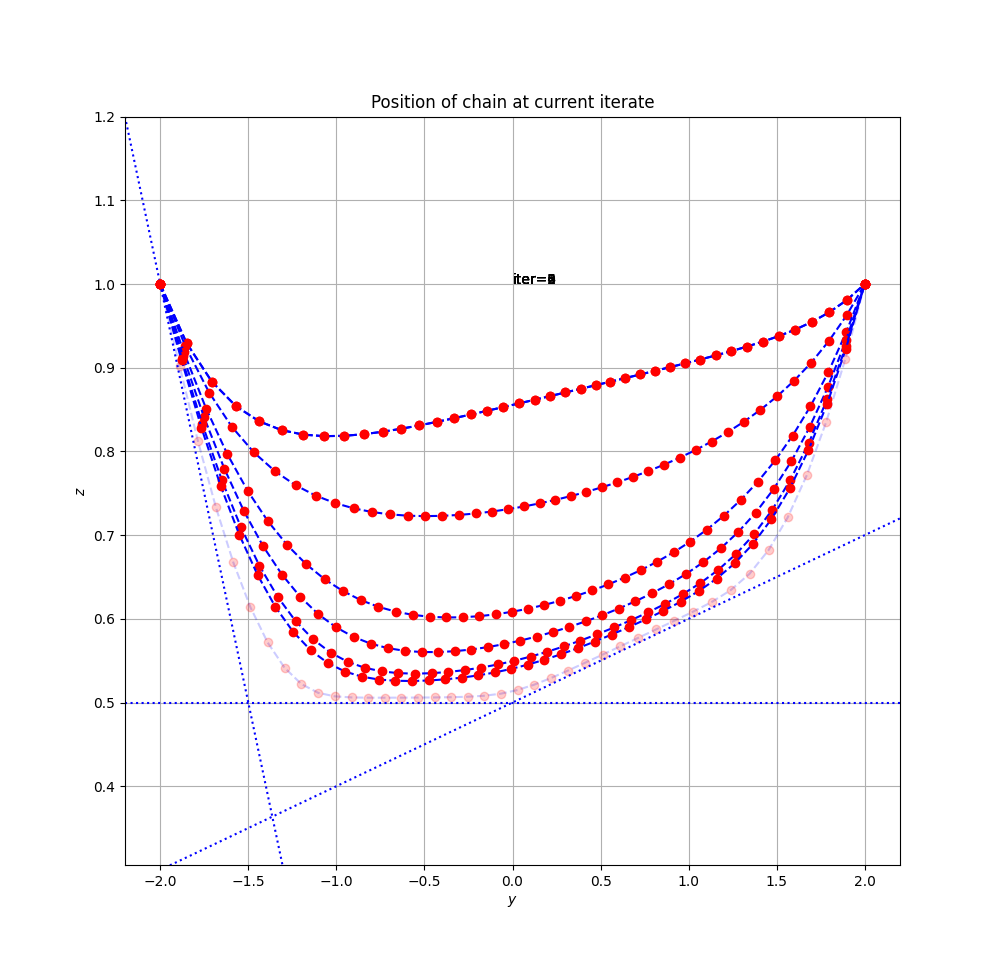
\includegraphics[width=\textwidth]{chain.png}
  \caption{Convergence of the inequality-constrained hanging chain problem using the Interior Point Method described in this exercise in $14$ iterations, illustrated by superposition of intermediate solutions. For Armijo-Backtracking, $\gamma=\frac{1}{4}, \beta=0.8$ was chosen. The code is shown in \autoref{sec:code}}
\end{figure}



\chapter{Sequential Quadratic Programming}
\equationnamedbox{Generic NLP}{
    \begin{align}
    \min_{x\in\mathds{R}^n} \quad & f(x)\\
    \text{s.t.}\quad & g(x) = 0\\
    & h(x) \geq 0
    \end{align}
}

\section{KKT-Conditions of generic NLP}
\begin{align}
    \nabla f(x) - \nabla h(x) \mu - \nabla g(x)\lambda &= 0\\
    g(x) &= 0\\
    h(x) &\geq 0\\
    \mu &\geq 0\\
    \forall i \in \mathds{N}_1^q: \quad \mu_i h_i(x) &= 0
\end{align}

\section{QP-subproblem at $x^{[k]}$}
Let $p\coloneq x-x^{[k]}$ and $B_k = \Laplace_x f\br{x^{[k]}}$. Linearize the constraints and approximate the objective by a quadratic form using Taylor expansion:

\equationnamedbox{QP-subproblem}{
    \begin{align*}
        \min_{p\in\mathds{R}^n} \quad & \nabla f(x)^T p + \frac{1}{2} p^T B_k p\\
        \text{s.t.}\quad & h\br{x^{[k]}} + \nabla h\br{x^{[k]}}^T p \geq 0\\
        & g\br{x^{[k]}} + \nabla g\br{x^{[k]}}^T p = 0
    \end{align*}
}

\section{Proofs}
TODO

\chapter{A sample exam question}
\equationnamedbox{Problem}{
    \begin{align}
    \min_{x\in\mathds{R}^2} \quad & x_2^4 + \br{x_1+2}^4\\
    \text{s.t.}\quad & x_1 - x_2 = 0\label{eq:prob-constr-eq}\\
    & x_1^2 + x_2^2 \geq 8\label{eq:prob-constr-ineq}
    \end{align}
}
\section{Variables and Constraints}
There are two scalar decision variables ($x_1, x_2$), one equality constraint (\autoref{eq:prob-constr-eq}) and one inequality constraint (\autoref{eq:prob-constr-ineq}).

\section{Sketch feasible set}
Imagine a $45\deg$ diagonal line (horizontal axis is $x_1$, vertical is $x_2$) through the origin and a circle of radius $\sqrt{8}$ around the origin, where the parts of the line inside the circle are highlighted and labelled as $\Omega$

\section{Standard Form}
\begin{align}
    f(x) &= x_2^4 + \br{x_1+2}^4\\
    g(x) &= x_1 - x_2\\
    h(x) &= 8 - x_1^2 - x_2^2
\end{align}
then:
\begin{align}
    \min_{x\in\mathds{R}^2} \quad & f(x)\\
    \text{s.t.}\quad & g(x)=0\\
    & h(x)\geq 0
    \end{align}


\section{Convexity}
The problem is convex.

$f(x)$ is convex in $x$, since \begin{align*}
    \nabla f(x) &= \begin{bmatrix}
        4(x_1+2)^3\\
        4x_2^3
    \end{bmatrix}\\
    \Laplace f(x) &= \begin{bmatrix}
        12(x_1+2)^2 & 0\\
        0 & 12x_2^2
    \end{bmatrix}\\
    \forall a,b,x_1,x_2\in\mathds{R}:\quad 
    \begin{bmatrix}a & b\end{bmatrix}
    \begin{bmatrix}
        12(x_1+2)^2 & 0\\
        0 & 12x_2^2
    \end{bmatrix}
    \begin{bmatrix}a\\b\end{bmatrix}
    &= 
    \underbrace{a^2}_{\geq 0} \cdot \underbrace{12(x_1+2)^2}_{\geq 0} + \underbrace{b^2}_{\geq 0}\cdot \underbrace{12x_2^2}_{\geq 0} \geq 0 
\end{align*}

$\Omega$ is convex since it is the intersection of two convex sets, namely a line defined by the affine equality constraint $g$ and a disk defined by $h$ (which is the level set of a convex quadratic function)

\section{Lagrangian}
\begin{align*}
    \mathcal{L}\br{x,\lambda,\mu} &= f(x) - \lambda^T g(x) - \mu^T h(x)\\
    &= 
    \underbrace{x_2^4 + \br{x_1+2}^4 }_{f(x)}
    \underbrace{-\lambda\br{x_1 - x_2}}_{- \lambda^T g(x)}
    \underbrace{- \mu\br{8 - x_1^2 - x_2^2}}_{- \mu^T h(x)}
\end{align*}

\section{Active set at $\bar{x}$}
At $\bar{x} = \begin{bmatrix}-2\\-2\end{bmatrix}$, the active set is $\mathcal{A} = \{1\}$ since the first and only inequality constraint is active ($h(\bar{x}) = 8-2^2-2^2=0$).

\section{LICQ at $\bar{x}$}

\begin{align}
    \nabla g(\bar{x}) &= \begin{bmatrix}1\\-1\end{bmatrix}\\
    \nabla h(\bar{x}) &= \begin{bmatrix}-2x_1\\-2x_2\end{bmatrix}
    = \begin{bmatrix}4\\4\end{bmatrix}\\
\end{align}

where $\nabla g(\bar{x}) \cdot \nabla h(\bar{x}) = 4-4 = 0 \Longrightarrow g(\bar{x}), h(\bar{x})$ are linearly independent, so LICQ holds at $\bar{x}$

\section{Active set at $x^*$}
At $x^* = \begin{bmatrix}-1\\-1\end{bmatrix}$ we have $h(x^*) = 8-1-1 = 6 > 0$, so the only inequality constraint is inactive and $\mathcal{A}\br{x^*}=\emptyset$

\section{LICQ at $x^*$}

Since $\mathcal{A}\br{x^*}=\emptyset$, it remains to show that $\left\{ \nabla g(x^*) \right\}$ is linearly independent, which is trivially true, so LICQ holds at $x^*$

\section{Tangent Cone at $x^*$}

\begin{align}
    T_{\Omega}\br{x^*} &= \left\{
       \forall x\in\mathds{R}^2 :\,
       x \cdot  \begin{bmatrix}1\\-1\end{bmatrix} = 0
       \,\middle |\, 
       x
    \right\}\\
    &= \left\{
       \forall t\in\mathds{R} \,\middle |\, 
       t \begin{bmatrix}1\\1\end{bmatrix}
    \right\}
\end{align}

\section{KKT-conditions at $x^*$}

The KKT-conditions using $\nabla f(x), \nabla g(x), \nabla h(x)$ as derived above read:

\begin{align}
    \begin{bmatrix}
        4(x_1+2)^3\\
        4x_2^3
    \end{bmatrix} - \begin{bmatrix}-2x_1\\-2x_2\end{bmatrix} \mu - \begin{bmatrix}1\\-1\end{bmatrix}\lambda &= 0\\
    x_1 - x_2 &= 0\\
    8 - x_1^2 - x_2^2 &\geq 0\\
    \mu &\geq 0\\
    \mu \br{8 - x_1^2 - x_2^2} &= 0
\end{align}

So at $x^* = \begin{bmatrix}-1\\-1\end{bmatrix}$:
\begin{align}
    \begin{bmatrix}4\\-4\end{bmatrix} 
    - \begin{bmatrix}2\\2\end{bmatrix} \mu 
    - \begin{bmatrix}1\\-1\end{bmatrix}\lambda &= 0\\
    -1 +1 &= 0\\
    6 &\geq 0\\
    \mu &\geq 0\\
    \mu \cdot 6 &= 0 \label{eq:kkt-mu-zero}
\end{align}

It follows from \autoref{eq:kkt-mu-zero} that $\mu=0$, which means that:
\begin{equation}
    \begin{bmatrix}4\\-4\end{bmatrix} 
    -\begin{bmatrix}1\\-1\end{bmatrix}\lambda = 0
\end{equation}
which implies $\lambda = 4$. 

All KKT-conditions are satisfied for $\mu^*=0, \lambda^* =4$

\section{SONC at $x^*$}

The SONC for $x^*$ are:
\begin{enumerate}
    \item $\exists \lambda^*, \mu^*$ such that KKT-conditions hold at $x^*$
    \item $\forall p\in C(x^*, \mu^*): p^T\Laplace_x \mathcal{L}(x^*,\lambda^*,\mu^*) p \geq 0$
\end{enumerate}

The former was shown in the previous answer, with $\lambda^* = 4, \mu^*=0$. The latter requires the critical cone:
\begin{align}
    C(x^*, \mu^*) &= \left\{ \forall p\in\mathds{R}^2: \nabla f(x^*) \cdot p = 0 \,\middle | \, p\right\}\\
    &= \left\{ \forall p\in\mathds{R}^2: \begin{bmatrix}4\\-4\end{bmatrix}  \cdot p = 0 \,\middle | \, p\right\}\\
    &= \left\{ \forall t\in\mathds{R}  \,\middle | \, \begin{bmatrix}t\\t\end{bmatrix} \right\}
\end{align}

We also need:
\begin{align}
    \mathcal{L}(x,\lambda^*,\mu^*) 
    &= 
    x_2^4 + \br{x_1+2}^4
    -\lambda^*\br{x_1 - x_2}
    \underbrace{- \mu^*\br{8 - x_1^2 - x_2^2}}_{=0 \text{ since } \mu^*=0}\\
    &=
    x_2^4 + \br{x_1+2}^4
    -\lambda^* x_1 -\lambda^* x_2\\
    \nabla_x \mathcal{L}(x,\lambda^*,\mu^*) &= 
    \begin{bmatrix}
        4(x_1+2)^3 - \lambda^*\\
        4x_2^3 - \lambda^*
    \end{bmatrix}\\
    \Laplace_x \mathcal{L}(x,\lambda^*,\mu^*) &= 
    \begin{bmatrix}
        12(x_1+2)^2 & 0\\
        0 & 12x_2^2
    \end{bmatrix}\\
    \Laplace_x \mathcal{L}(x^*,\lambda^*,\mu^*) &= 
    \begin{bmatrix}
        12 & 0\\
        0 & 12
    \end{bmatrix} = 12\mathds{I}
\end{align}

to show that for all $p\in C(x^*, \mu^*)$:
\begin{align}
    p^T\Laplace_x \mathcal{L}(x^*,\lambda^*,\mu^*) p
    &=  \begin{bmatrix}t & t\end{bmatrix} \br{12\mathds{I}} \begin{bmatrix}t \\ t\end{bmatrix}\\
     &=  \begin{bmatrix}t & t\end{bmatrix} \begin{bmatrix}12t \\ 12t\end{bmatrix}\\
     &= 12t^2 + 12t^2 \\
     &= 24t^2 \geq 0
\end{align}

so $x^*$ fulfills  SONC. 


Also, since $C(x^*, \mu^*)\backslash\{\vec{0}\} = \left\{ t\in\mathds{R}: t\neq 0 \,\middle | \, \begin{bmatrix}
t\\t
\end{bmatrix}\right\}$ and $t\neq 0 \implies 24t^2 > 0$ and SONC hold, it follows that SOSC hold, so $x^*$ is a strict local minimizer. 

Since $x^*$ is a \textit{strict} local minimizer of a convex problem, this actually implies that $x^*$ is the global minimum.

\chapter{Code}\label{sec:code}

\inputminted{python}{hanging_chain_ip.py}

\end{document}